\documentclass[11pt]{article}

\usepackage[margin=1in]{geometry}
\usepackage{lmodern}
\usepackage[T1]{fontenc}
\usepackage{amsmath,amssymb}
\usepackage{booktabs}
\usepackage{graphicx}
\usepackage{microtype}
\usepackage[colorlinks=true,linkcolor=blue!55!black,citecolor=blue!55!black,urlcolor=blue!55!black]{hyperref}
\usepackage[numbers,sort&compress]{natbib}
\usepackage{caption}
\usepackage{subcaption}
\usepackage{enumitem}
\usepackage{xcolor}

\captionsetup{font=small,labelfont=bf}
\setlist[itemize]{leftmargin=1.4em,itemsep=1pt,topsep=2pt}

\newcommand{\unknown}{\texttt{unknown}}
\newcommand{\punk}{p(\unknown)}
\newcommand{\ie}{i.e.,\ }
\newcommand{\eg}{e.g.,\ }

\title{\bfseries The Evidence Gate:\\[2pt]
How Vision-Language Models Decide to Answer Without Evidence}

\author{yuanchongbit}

\date{October 2026}

\begin{document}
\maketitle

\begin{abstract}
Vision-language models often assert an answer when the image does not contain the queried evidence, yet retract a correct answer as soon as a sentence in the prompt contradicts it. Are these failures of seeing, or of reporting what was seen? We introduce a $2\times3$ within-subject design---visual evidence $\{$present, verified absent$\}$ $\times$ textual hint $\{$none, correct, conflicting$\}$---built without editing a single pixel: ``absent'' is an object category that COCO's instance annotations and an independent presence probe both place outside the photograph. Across 261 verified samples and three models, the model's native output signals collapse under conflict ($\punk$ AUROC $0.993\to0.834$ on Qwen2.5-VL-3B; maximum probability falls below chance), while a linear probe on the final hidden state is unchanged ($0.995\to0.998$) and transfers across hints ($0.969$). A learned readout over the full 12-way distribution degrades less ($0.982\to0.923$), so the collapse is specific to the signals the model itself exposes, not to every function of its logits. Signal detection locates the failure: under conflict sensitivity collapses in all three models ($d'=3.51\to1.45$, $2.98\to1.24$, $3.44\to1.44$), while criterion shifts are inconsistent in sign; a correct hint never reduces sensitivity. The conflict compresses the evidence axis rather than lowering a threshold. Layer-wise activation patching locates the suppression late: restoring the unpolluted state recovers $80\%$ of the lost refusal at $89\%$ depth in the 3B model, $90\%$ at $93\%$ in the 7B model, and $93\%$ at $93\%$ in LLaVA-OneVision-7B, a second model family. A difference-of-means direction is causally sufficient and partly necessary, with a monotone dose--response on held-out scenes. As a consequence, a training-free probe gate reduces fabrication at $50\%$ coverage from $0.249$ to $0.011$. External validation on VizWiz and VQA-v2 reproduces the behavioural asymmetry and bounds the claim: on naturally unanswerable images the model's own $\punk$ is as good as the probe, so internal gating helps specifically when a hint attacks the refusal gate. The code, the frozen benchmark and all result summaries are released.
\end{abstract}

\section{Introduction}

Ask a vision-language model (VLM) \emph{``What color is the umbrella?''} about a photograph with no umbrella, and it will usually answer \unknown. Prepend one plausible sentence---\emph{``Hint: the umbrella is black.''}---and the same model answers \emph{black} with high confidence. The failure is not that the model cannot see. The object was never there.

Two literatures describe adjacent phenomena. Work on hallucination measures objects a model reports but the image does not contain \citep{rohrbach2018object,li2023pope}. Work on sycophancy measures answers that follow a user's stated belief rather than the input \citep{sharma2023sycophancy,turpin2023language,hong2026tosee}. Both describe behaviour; neither separates two questions that the behaviour confounds: \emph{is the evidence represented?} and \emph{is the decision to abstain driven by that representation?} A model that answers \emph{black} may have lost the evidence, or it may still represent ``no umbrella'' while a later stage overrides abstention.

We separate the two with a design in which the image is held fixed and only the \emph{epistemic status} of the question changes. Each of 261 photographs appears in six cells: the queried object is present or annotated-absent, crossed with no hint, a correct hint, or a conflicting hint. The absent arm requires no image editing: it asks about an object category that COCO's instance annotations place outside the image. Every cell therefore shares the same pixels, and the six prompts differ only in what they assert. A separate yes/no probe confirms that the absent objects really are absent.

The design yields a sharp dissociation (Figure~\ref{fig:signals}). With no hint, the model's own $\punk$ detects evidence availability almost perfectly (AUROC $0.993$), so there is no room for a better internal signal. Under a conflicting hint, every output-space signal degrades: $\punk$ drops to $0.834$, maximum probability to $0.463$---below chance---and a learned readout over the full 12-way distribution reaches only $0.923$. A linear probe on the final-token hidden state, trained only on the no-hint pair, does not move ($0.998$) and transfers to the conflicting pair at $0.969$. The conflict changes what the model \emph{says about its evidence}, not what it \emph{knows about its evidence}.

Two causal interventions show that this is not a correlational artefact. Along the probe direction, adding or ablating a single vector changes abstention bidirectionally and dose-monotonically, including on scenes held out from fitting. Pasting the no-hint state back at intermediate layers recovers the lost refusal, and the recovery profile is steep and late: little at two-thirds depth, most of it in the final few layers. The same profile appears on Qwen2.5-VL-3B, Qwen2.5-VL-7B and LLaVA-OneVision-7B. The last model is far more hint-sensitive than either Qwen model, yet the suppression is written at the same relative depth---sensitivity and locus are separable.

Finally, we turn the mechanism into a training-free gate: rank items by the internal probe and answer only the top fraction. At $50\%$ coverage under conflict, fabrication falls from $0.249$ ($\punk$) to $0.011$ (probe). The benefit is specific to the polluted regime. On naturally unanswerable VizWiz questions the model's own $\punk$ matches the frozen probe, and on VQA-v2 colour questions the probe's ordering is preserved but its calibration is not. We report both boundaries rather than hiding them.

\paragraph{Contributions.}
\begin{itemize}
\item \textbf{A controlled construction.} A $2\times3$ within-subject benchmark with no image editing, in which ``evidence absent'' is verified by annotations and by an independent presence probe, and in which the hint is plausible rather than adversarial. The 261-item manifest and verified labels are frozen and released.
\item \textbf{A mechanistic dissociation with causal support.} The model's native output signals collapse under conflict while the internal evidence representation remains linearly decodable. Steering and layer-wise patching establish sufficiency, partial necessity, and a late-write locus, replicated on three models from two families.
\item \textbf{A deployable consequence and its boundary.} A training-free probe gate reduces fabrication under conflict by more than an order of magnitude, and external validation identifies when this advantage disappears.
\end{itemize}

\section{Related Work}

\paragraph{Sycophancy and prompt-induced error.}
Language models shift answers toward a user's stated view \citep{sharma2023sycophancy}, and their explanations can diverge from the evidence that actually drove the answer \citep{turpin2023language}. Recent work documents the multimodal version: VLMs change visual answers to agree with textual assertions, sometimes while still encoding the original content, and \citet{hong2026tosee} establish this representation--output dissociation correlationally across nine VLMs. Our contribution is not another measurement of the effect but a causal decomposition: steering and patching establish which stage the hint acts on, and the resulting direction supports a training-free gate.

\paragraph{Abstention and selective prediction.}
Selective prediction trades coverage for risk using a confidence score \citep{geifman2017selective}. For VQA, learned abstention and selective answering have been studied under distribution shift and on unanswerable questions \citep{whitehead2022reliable,srinivasan2024selective}. These methods ask \emph{which} scalar to threshold. We ask \emph{which representation} the scalar should be computed from, and show that the model's own abstention probability is the wrong representation precisely when a hint is present.

\paragraph{Probing and steering internal states.}
Linear probes recover truthfulness, knowledge and uncertainty from hidden states \citep{alain2016understanding,azaria2023internal,burns2023discovering,kadavath2022language,marks2024geometry}. Difference-of-means directions can steer behaviour \citep{turner2023activation,rimsky2024steering,zou2023representation,li2023inference}, and refusal in chat models is mediated by a low-dimensional direction \citep{arditi2024refusal}, though not exclusively so \citep{joad2026more}. Activation steering has also been applied to VLM refusal \citep{yang2026steering}. We study a different axis---whether the \emph{evidence} needed to answer is available---and connect the direction to a layer-resolved account of where the hint overrides it.

\paragraph{Localisation.}
Activation patching replaces a state in one forward pass with a state from another and measures the effect on the output \citep{meng2022locating}. We use it with a same-sample source and a shuffled-source control to locate, not to quantify, the stage at which the conflict is written.

\paragraph{Hallucination in VLMs.}
Object hallucination is typically measured by asking about objects that are absent \citep{rohrbach2018object,li2023pope}. We adopt the logic of absent-object questions but make the comparison within-image and within-question, vary only the textual assertion, and add an internal readout. The resulting benchmark is small by hallucination standards (261 items) but densely observed: six conditions per image plus probes and interventions.

\section{Design and Data}

\subsection{The $2\times3$ design}

Each sample is a photograph, a queried category $c$, and a gold colour $g$. The six conditions are shown in Figure~\ref{fig:design}.
\begin{center}
\begin{tabular}{llll}
\toprule
 & \multicolumn{3}{c}{textual hint} \\
\cmidrule(lr){2-4}
visual evidence & none & correct & conflicting \\
\midrule
object present & \texttt{sufficient|none} & \texttt{sufficient|correct} & \texttt{sufficient|wrong} \\
object absent & \texttt{absent|none} & \texttt{absent|a} & \texttt{absent|b} \\
\bottomrule
\end{tabular}
\end{center}
In the present arm the correct hint states $g$ and the conflicting hint states a fixed far-hue distractor. In the absent arm there is no correct colour; \texttt{a} is the absent category's most frequent colour in COCO val, and \texttt{b} is its second most frequent colour. The two absent hints therefore differ in plausibility but both assert a colour for an object that is not in the image. Every image appears in all six cells, so all comparisons are within-image and within-question.

\begin{figure}[t]
\centering
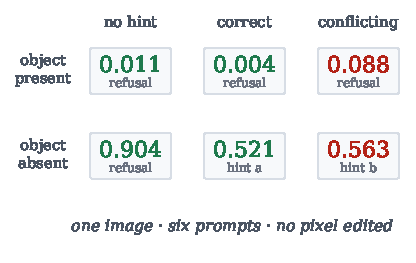
\includegraphics[width=\linewidth]{figures/fig_design.pdf}
\caption{The $2\times3$ design. Each image appears in all six cells; the absent arm asks about a category with no annotation in the image. Numbers are refusal rates from Table~\ref{tab:behaviour}.}
\label{fig:design}
\end{figure}


\subsection{Construction without image editing}

Starting from COCO val2017 \citep{lin2014coco}, we retain single annotated instances with box short side $\ge 44$ px, area fraction $1.5$--$35\%$, and mask/box fill $\ge 0.45$. Colour is proposed as the area-dominant colour inside the instance mask, with purity and margin gates, then verified by hand on contact sheets. Of 1447 geometric candidates, 413 passed the automatic colour gate and 261 survived manual verification (blue 88, white 79, black 45, green 25, red 15, yellow 9).

For the absent arm we sample a category with no annotation in the image (74 distinct categories) and use that category's $\{$first, second$\}$ most frequent colour in val as the hint. The hint is thus something a knowledgeable annotator might say, not an impossible string. No pixel is edited; the same JPEG is used in all six cells.

\paragraph{Manipulation check.}
A separate yes/no question (``Is there a $c$ in this image?'') yields mean $p(\text{yes})=0.095$ on 260 category-matched negative images versus $p(\text{yes})=0.95$ on the original images. The absent arm is verified absent independently of the colour question, which presupposes the object.

\subsection{Prompts and readout}

The system prompt asks for one word and instructs the model to answer \unknown\ when the image does not contain enough information. The user prompt is
\begin{quote}\small
\ttfamily
[Hint: the \{category\} is \{colour\}.]\newline
What color is the \{category\}?\newline
Answer with one word.
\end{quote}
where the hint line is omitted in the no-hint condition. The readout is a distribution over the eleven colour words plus \unknown; all twelve candidates are single tokens in every tokenizer used. Probabilities are the softmax over their logits at the first answer position.

\subsection{Signals}

\paragraph{Output signals.} We compute $\punk$, maximum probability, the top-two gap, negative entropy, and a 12-dimensional logistic readout over the full candidate distribution. These use exactly the same forward pass as the answer.

\paragraph{Internal probe.} A logistic regression on the final-token hidden state (2048-d for the 3B model, 3584-d for the 7B models), trained on the no-hint pair \texttt{sufficient|none} vs.\ \texttt{absent|none} and evaluated on hinted pairs. Cross-validation is grouped by sample (five folds) so a scene never appears in both train and test; a second analysis groups by queried category to test for a category$\to$colour shortcut. Regularisation strength is chosen by cross-validation. The probe is frozen when transferred to external data.

\paragraph{Steering.} The direction $w$ is the difference of class means on the no-hint pair. We inject $\alpha\lVert h\rVert w$ at the final position, where $\lVert h\rVert$ is the median hidden-state norm and $\alpha\in\{\pm0.25,\pm0.5\}$, and ablate by projecting $w$ out of the state. A split-half check fits $w$ on 130 scenes and evaluates on the remaining 131.

\paragraph{Patching.} For layer $L$ we capture the final-token state from a no-hint forward pass and paste it into the hinted pass at the same layer, letting the remaining layers run. A shuffled-source control pastes another sample's no-hint state at the same layer. Since pasting changes the state distribution, we use patching for localisation and rely on steering for quantitative effect size.

\paragraph{Metrics.} Evidence detection is AUROC over the 522 paired items, with grouped bootstrap confidence intervals (2000 resamples, groups = samples) and paired bootstrap intervals for differences between signals. Selective answering is reported as fabrication rate at fixed coverage: among the top-$k$ items ranked by an evidence score, the fraction that are absent-object items answered with a colour. Fabrication at $50\%$ coverage is the primary operating point.

\paragraph{Models.} Qwen2.5-VL-3B and 7B \citep{bai2025qwen25vl} in bfloat16 with SDPA attention and at most $1024^2$ pixels, and LLaVA-OneVision-7B \citep{li2024llavaov} resized to 768 px, loaded through \texttt{AutoModelForImageTextToText}. All experiments ran on a single 24 GB A10.

\section{Results}

\subsection{Behaviour: hints move both arms in opposite directions}

\begin{table}[t]
\centering
\small
\caption{Behaviour on 261 verified samples (Qwen2.5-VL-3B). ``Adopts hint'' is the fraction whose argmax equals the hinted colour. UAR is answering when the object is absent; OAR is refusing when it is present.}
\label{tab:behaviour}
\begin{tabular}{lccccc}
\toprule
condition & refusal & mean conf. & adopts hint & accuracy & $n$ \\
\midrule
present $\cdot$ correct hint & 0.004 & 0.943 & --- & 0.973 & 261 \\
present $\cdot$ conflicting hint & 0.088 & 0.674 & 0.448 & 0.383 & 261 \\
present $\cdot$ no hint & 0.011 & 0.836 & --- & 0.762 & 261 \\
absent $\cdot$ hint a & 0.521 & 0.699 & 0.467 & --- & 261 \\
absent $\cdot$ hint b & 0.563 & 0.707 & 0.433 & --- & 261 \\
absent $\cdot$ no hint & 0.904 & 0.799 & --- & --- & 261 \\
\bottomrule
\end{tabular}
\end{table}

Table~\ref{tab:behaviour} shows the basic pattern. Without hints the model is conservative in the right way: it refuses $90.4\%$ of absent-object questions and only $1.1\%$ of present-object ones. A conflicting hint moves both arms in the direction of the assertion: refusal on the absent arm falls to $52$--$56\%$, and $43$--$47\%$ of answers are the hinted colour. The same hint also makes the present arm refuse more often ($1.1\%\to8.8\%$) and drops accuracy from $76.2\%$ to $38.3\%$. A correct hint does the opposite, raising accuracy to $97.3\%$. The hint is therefore treated as evidence, not as noise: it helps when true and hurts when false, which is what makes the conflicting condition a causal manipulation of the evidence variable.

\subsection{Output signals collapse; the internal representation does not}
\label{sec:signals}

\begin{table}[t]
\centering
\small
\caption{Evidence detection (AUROC over 522 paired items) for signals computed from the same forward pass. The probe is a linear classifier on the final hidden state. Brackets are grouped bootstrap $95\%$ CIs.}
\label{tab:signals}
\begin{tabular}{lcccc}
\toprule
condition pair & final-state probe & $\punk$ & max probability & 12-d logit probe \\
\midrule
present vs.\ absent, no hint & 0.995 [0.989, 0.999] & \textbf{0.993} & 0.615 & 0.982 \\
present$\cdot$conflict vs.\ absent$\cdot$hint & \textbf{0.998} [0.994, 1.000] & 0.834 & 0.463 & 0.923 \\
present$\cdot$correct vs.\ absent$\cdot$hint & \textbf{0.997} [0.994, 0.999] & 0.969 & 0.916 & 0.974 \\
\bottomrule
\end{tabular}
\end{table}

Table~\ref{tab:signals} and Figure~\ref{fig:signals} contain the central result. With no hint, $\punk$ is already an excellent evidence detector ($0.993$), statistically indistinguishable from the probe ($+0.002$ $[-0.003,+0.007]$). The interesting regime is conflict. There $\punk$ loses $0.159$ AUROC, maximum probability loses $0.152$ and ends below chance, and even a learned readout over the entire output distribution loses $0.059$. The hidden-state probe loses $0.003$ in the other direction, and its advantage over $\punk$ becomes $+0.164$ $[+0.132,+0.196]$. Training the probe on no-hint pairs and testing on conflicting pairs gives $0.969$; the reverse transfer is $0.999$.

The same pattern holds under a correct hint, where no signal collapses: the probe reaches $0.997$ and $\punk$ $0.969$. This rules out a trivial explanation in which the probe merely responds to the presence of a hint string. What matters is whether the hint conflicts with the image.

\subsection{Conflict compresses the evidence axis}

A natural reading of Table~\ref{tab:behaviour} is that a conflicting hint lowers the refusal threshold: the model becomes more willing to answer. Signal detection separates this from a loss of sensitivity. Using the out-of-fold probe score as the evidence axis, we compute $d'$ and criterion $c$ for each condition, and fit the psychometric model $\mathrm{logit}\,P(\text{refuse})=b_0+az+\sum_k d_k(b_k+a_kz)$ over the 1{,}827 item--condition observations. For the fit, $z$ is taken from the \emph{no-hint} forward pass of the same item, so the hint cannot move the axis it is compared on.

\begin{table}[t]
\centering
\small
\caption{Signal detection. $d'$ and $c$ are computed from refusal rates on the paired present/absent items. The last three columns are from the parametric fit: logit slope on the no-hint probe score, and predicted refusal at the median no-hint score of absent ($z=-8.56$) and present ($z=7.43$) items.}
\label{tab:sdt}
\begin{tabular}{lccccc}
\toprule
condition & $d'$ & $c$ & slope & $P(\text{refuse})$ absent & present \\
\midrule
no hint & 3.51 & 0.46 & $-0.719$ & 0.988 & 0.001 \\
conflicting hint & 1.45 & 0.62 & $-0.171$ & 0.577 & 0.082 \\
correct hint & 3.83 & 0.62 & $-0.680$ & 0.983 & 0.001 \\
\bottomrule
\end{tabular}
\end{table}

Table~\ref{tab:sdt} shows the dissociation. Under conflict, sensitivity falls from $3.51$ to $1.45$ ($\Delta d'=-2.13$ $[-2.69,-1.66]$), while the criterion does not move reliably ($\Delta c=+0.16$ $[-0.18,+0.39]$). A correct hint leaves both unchanged ($\Delta d'=+0.31$ $[-0.36,+0.93]$; $\Delta c=+0.16$ $[-0.18,+0.46]$). The behavioural effect is bidirectional: conflict raises refusal on present items ($1.1\%\to8.8\%$) and lowers it on absent items ($90.4\%\to54.2\%$). A criterion shift moves both arms in the same direction, so it cannot produce this pattern.

The parametric fit makes the compression explicit. The conflict slope is $-0.171$ against $-0.719$ (change $+0.548$ $[0.439,0.774]$; likelihood-ratio $178.2$, $df=2$, $p<10^{-38}$), a fourfold flattening. The fitted curve reproduces both arms: at the median evidence of absent items, refusal falls from $98.8\%$ to $57.7\%$; at the median of present items, it rises from $0.1\%$ to $8.2\%$. A correct hint leaves the curve intact (slope change $+0.039$ $[-0.074,0.196]$). The change is a pivot, not a translation: the two curves cross near $z=-1.2$. This is the behavioural counterpart of Section~\ref{sec:signals}: the evidence is still linearly decodable from the same hidden states at $0.998$ AUROC, but the decision uses it with much lower sensitivity. The failure is in the use of evidence, not in its representation.

\begin{table}[t]
\centering
\small
\caption{Sensitivity and criterion under conflict in the three models ($n=261$ scenes each; 522 absent items in the conflict condition). Paired differences versus the no-hint condition, with cluster-bootstrap $95\%$ CIs over scenes.}
\label{tab:sdt-cross}
\begin{tabular}{lcccc}
\toprule
model & $d'$ no hint & $d'$ conflict & $\Delta d'$ & $\Delta c$ \\
\midrule
Qwen2.5-VL-3B & 3.51 & 1.45 & $-2.13$ $[-2.69,-1.66]$ & $+0.16$ $[-0.18,+0.39]$ \\
Qwen2.5-VL-7B & 2.98 & 1.24 & $-1.80$ $[-2.14,-1.39]$ & $-0.54$ $[-0.73,-0.35]$ \\
LLaVA-OneVision-7B & 3.44 & 1.44 & $-2.06$ $[-2.71,-1.32]$ & $+1.00$ $[+0.66,+1.33]$ \\
\bottomrule
\end{tabular}
\end{table}

The sensitivity collapse replicates in all three models (Table~\ref{tab:sdt-cross}). The criterion does not: its shift is null in the 3B model, negative in the 7B model and positive in LLaVA. A uniform lowering of the refusal threshold predicts a common direction, so the cross-model pattern argues against a criterion account. It also warns against over-reading $c$: the equal-variance estimate is biased when $d'$ changes, which is why we treat the consistent $d'$ loss, not the sign of $\Delta c$, as the invariant. Under a correct hint $d'$ never falls ($\Delta d'=+0.31$ $[-0.36,+0.93]$, $+0.50$ $[+0.17,+0.82]$, $+0.32$ $[0.00,+0.68]$), so the loss is specific to conflict.

\begin{figure}[t]
\centering
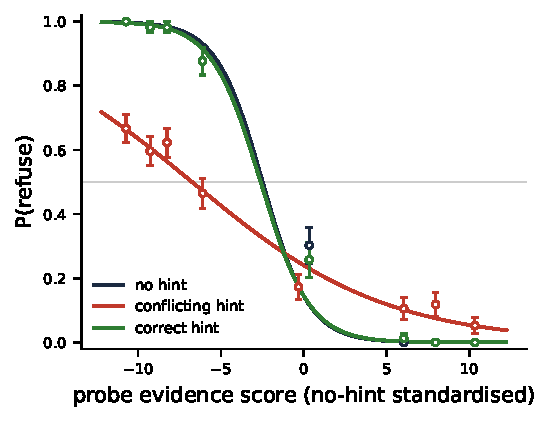
\includegraphics[width=0.52\linewidth]{figures/fig_sdt.pdf}
\caption{Refusal probability as a function of the no-hint probe score, which is measured before the hint is applied. Points are binned rates with binomial standard errors; lines are the fitted psychometric curves. The conflicting-hint curve is four times flatter and pivots around $z\approx-1.2$; the correct-hint curve tracks the no-hint curve.}
\label{fig:sdt}
\end{figure}

\subsection{Controls: the probe reads the image, not the prompt}

Three controls address the concern that the probe separates the two arms from text alone. First, a gray image with the same prompts and the same dimensions yields probe AUROC $0.849$ / $0.981$ / $0.930$ under no / conflicting / correct hints, and $\punk$ $0.700$ / $0.325$ / $0.433$. Text alone carries some category$\to$common-colour prior, enough to reach $0.85$ on the no-hint pair. But the direction learned from gray images transfers across hints at only $0.540$ / $0.603$, whereas the direction learned from real images transfers at $0.969$ / $0.996$. The real-image direction is shared across prompts; the text-prior direction is not.

Second, we construct category-matched pairs. Each present image is paired with another image from the same pool in which the queried category is annotated absent; both sides receive exactly the same prompt, and one side is the positive. The two sides come from the same geometric filter, so scene statistics are matched. Cross-validation groups by category, so a held-out fold contains categories never seen during fitting. The probe reaches $0.985$ with no hint and $0.973$ under conflict; $\punk$ drops from $0.983$ to $0.817$ and maximum probability from $0.701$ to $0.468$. On these 260 negative images, the presence probe gives mean $p(\text{yes})=0.095$. A pure category prior cannot explain a probe that generalises to unseen categories with the question held fixed.

Third, the main probe analysis grouped by sample already prevents scene leakage. Repeating it with folds grouped by queried category gives $0.995$ / $0.997$ / $0.996$ for the three condition pairs and transfers of $0.969$ / $0.996$, essentially unchanged.

\begin{figure}[t]
\centering
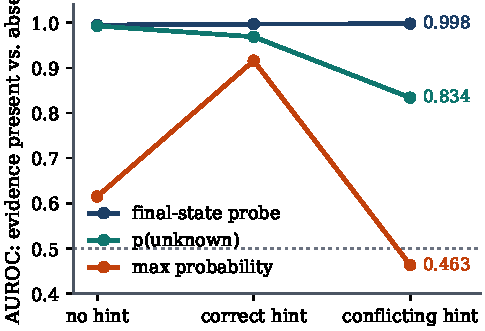
\includegraphics[width=0.62\linewidth]{figures/fig_signals.pdf}
\caption{Evidence detection under three hint conditions. All output-space signals degrade under conflict; the final-state probe does not. Values are AUROC over the 522 paired items; the dotted line is chance.}
\label{fig:signals}
\end{figure}

\subsection{The direction is causally sufficient and partly necessary}

\begin{table}[t]
\centering
\small
\caption{Steering along the difference-of-means direction. $\alpha$ is a fraction of the median hidden norm; positive $\alpha$ pushes toward ``evidence present''. The lower block refits the direction on 130 scenes and evaluates only on the held-out 131.}
\label{tab:steer}
\begin{tabular}{lcccc}
\toprule
 & \multicolumn{2}{c}{present} & \multicolumn{2}{c}{absent} \\
\cmidrule(lr){2-3}\cmidrule(lr){4-5}
setting & refusal & top-1 conf. & refusal & adopts hint \\
\midrule
\multicolumn{5}{l}{\emph{In-sample direction ($n=261$)}}\\
base & 0.011 & 0.836 & 0.904 & 0.096 \\
ablate $w$ & 0.004 & 0.838 & 0.759 & 0.241 \\
$-0.50\,w$ & 0.352 & 0.741 & 0.989 & 0.011 \\
$-0.25\,w$ & 0.130 & 0.760 & 0.973 & 0.027 \\
$+0.25\,w$ & 0.000 & 0.878 & 0.330 & 0.670 \\
$+0.50\,w$ & 0.000 & 0.876 & 0.000 & 1.000 \\
\midrule
\multicolumn{5}{l}{\emph{Held-out half ($n=131$)}}\\
base & 0.015 & --- & 0.908 & --- \\
ablate $w$ & 0.008 & --- & 0.786 & --- \\
$-0.50\,w$ & 0.450 & --- & 0.992 & --- \\
$+0.25\,w$ & 0.000 & --- & 0.305 & --- \\
$+0.50\,w$ & 0.000 & --- & 0.000 & --- \\
\bottomrule
\end{tabular}
\end{table}

Table~\ref{tab:steer} shows that adding $w$ makes the model answer absent-object questions and subtracting it makes the model refuse present-object questions. The effect is monotone in $\alpha$ and saturates at both ends. Ablating $w$ lowers absent-object refusal from $0.904$ to $0.759$, so the direction is not merely sufficient: when the model has no hint to rely on, removing it removes part of the refusal. At the same time, present-object top-1 confidence stays between $0.741$ and $0.878$ across the sweep. The intervention moves the answer/refuse decision, not the entire representation.

The lower block refits $w$ on half the scenes and evaluates on the other half. The dose--response survives with slightly larger amplitudes at the extremes, consistent with a direction that is not overfitted to the evaluation items.

\subsection{The suppression is written in the last few layers}

\begin{figure}[t]
\centering
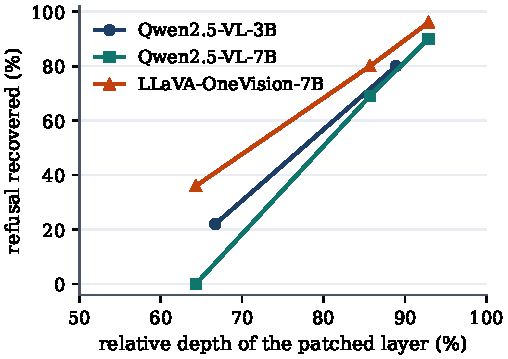
\includegraphics[width=0.62\linewidth]{figures/fig_depth.pdf}
\caption{Recovery of the refusal lost under conflict when the no-hint state is pasted back at layer $L$. Depth is relative to the model's decoder depth. The profile is late and steep in all three models; LLaVA is more hint-sensitive but not earlier.}
\label{fig:depth}
\end{figure}

\begin{table}[t]
\centering
\small
\caption{Layer-wise patching. ``Same'' pastes this sample's no-hint state at layer $L$; refusal and $\punk$ are measured after the remaining layers run. Recovery is relative to the no-hint and conflicting baselines of the same run.}
\label{tab:patch}
\begin{tabular}{llccc}
\toprule
model & source & refusal & $\punk$ & recovery \\
\midrule
Qwen2.5-VL-3B (36 layers) & no hint & 0.904 & 0.762 & 100\% \\
 & conflict & 0.521 & 0.470 & 0\% \\
 & same, L24 (67\%) & 0.594 & 0.535 & 22\% \\
 & same, L32 (89\%) & 0.839 & 0.704 & 80\% \\
\midrule
Qwen2.5-VL-7B (28 layers) & no hint & 0.958 & 0.899 & 100\% \\
 & conflict & 0.877 & 0.783 & 0\% \\
 & same, L18 (64\%) & 0.893 & 0.782 & 0\% \\
 & same, L24 (86\%) & 0.962 & 0.863 & 69\% \\
 & same, L26 (93\%) & 0.962 & 0.888 & 90\% \\
\midrule
LLaVA-OneVision-7B (28 layers) & no hint & 0.751 & 0.579 & 100\% \\
 & conflict & 0.161 & 0.194 & 0\% \\
 & same, L18 (64\%) & 0.314 & 0.299 & 27\% \\
 & same, L24 (86\%) & 0.648 & 0.480 & 74\% \\
 & same, L26 (93\%) & 0.743 & 0.550 & 93\% \\
\bottomrule
\end{tabular}
\end{table}

If the conflict erased the evidence, restoring an early state should not help. If it overrides a late decision, restoring a late state should. Table~\ref{tab:patch} and Figure~\ref{fig:depth} show the latter. In the 3B model, patching at layer 24 (67\% depth) recovers $22\%$ of the lost refusal; patching at layer 32 (89\%) recovers $80\%$. In the 7B model, layer 18 (64\%) recovers essentially nothing, layer 24 (86\%) recovers $69\%$, and layer 26 (93\%) recovers $90\%$. The suppression is concentrated in the final few layers, not spread through the network.

The shuffled-source control recovers as much or more (3B L32: $0.927$ refusal; 7B L26: $0.965$; LLaVA L26: $0.781$). Pasting another sample's no-hint state works, which means the patched state carries a category-level ``no evidence'' status rather than a sample-specific code. It also means the control cannot be used to estimate a clean effect size: replacing a state with a differently distributed one perturbs the residual stream. We therefore use patching to locate the stage and steering to quantify the effect.

LLaVA-OneVision-7B is the strongest test of generality. Its refusal under conflict is $0.161$, far lower than Qwen-7B's $0.877$: the same kind of hint is much more effective on this model. Yet the recovery profile is the same shape and the same depth ($27\%$, $74\%$, $93\%$). A model that is easier to fool does not have an earlier gate; its gate is pushed further open at the same place. This separates hint sensitivity from the locus of suppression.

\subsection{A training-free gate}

\begin{figure}[t]
\centering
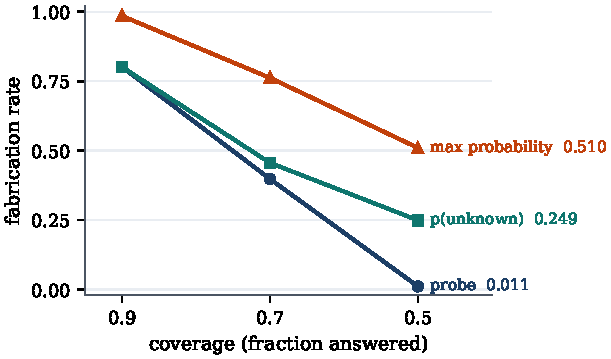
\includegraphics[width=0.62\linewidth]{figures/fig_risk.pdf}
\caption{Fabrication rate versus coverage under conflicting hints (Qwen2.5-VL-3B). Ranking by the internal probe removes most fabrications at moderate coverage; the model's own $\punk$ and maximum probability do not.}
\label{fig:risk}
\end{figure}

\begin{table}[t]
\centering
\small
\caption{Fabrication rate at fixed coverage under conflicting hints (Qwen2.5-VL-3B, out-of-fold scores). ``Probe'' ranks by the internal evidence score.}
\label{tab:gate}
\begin{tabular}{lccc}
\toprule
coverage & probe & $\punk$ & max probability \\
\midrule
50\% & \textbf{0.011} & 0.249 & 0.510 \\
70\% & \textbf{0.398} & 0.456 & 0.762 \\
90\% & 0.801 & 0.801 & 0.985 \\
\bottomrule
\end{tabular}
\end{table}

The mechanistic result suggests a simple gate: answer only if an internal evidence score is high. Table~\ref{tab:gate} and Figure~\ref{fig:risk} evaluate this with out-of-fold probe scores. At $50\%$ coverage under conflict, fabrication falls from $0.249$ to $0.011$, a $23\times$ reduction; maximum probability is worse than chance, at $0.510$. At $70\%$ coverage the probe hits the structural floor: answering $70\%$ of a set that is half absent requires answering at least $40\%$ of absent items, which is exactly what it achieves ($0.398$). The gate is therefore most useful at moderate coverage, where abstention is still allowed to be selective.

The same pattern appears on the other models: at $50\%$ coverage under conflict, probe $0.019$ versus $\punk$ $0.268$ on Qwen2.5-VL-7B, and $0.019$ versus $0.295$ on LLaVA-OneVision-7B.

\subsection{Task-form boundaries}

\begin{table}[t]
\centering
\small
\caption{The same images and absent categories with three question forms. The gate opens in all three; the output readout collapses only for colour.}
\label{tab:tasks}
\begin{tabular}{llccccc}
\toprule
task & condition & refusal & adopts hint & probe & $\punk$ & max prob. \\
\midrule
colour & present, no hint & 0.011 & --- & 0.995 & 0.993 & 0.615 \\
 & present, conflict & 0.088 & 0.448 & 0.997 & 0.834 & 0.463 \\
 & absent, no hint & 0.904 & --- & & & \\
 & absent, hint & 0.521 & 0.467 & & & \\
\midrule
side & present, no hint & 0.000 & --- & 0.993 & 0.989 & 0.791 \\
 & present, conflict & 0.000 & 0.268 & 0.991 & 0.966 & 0.744 \\
 & absent, no hint & 0.621 & --- & & & \\
 & absent, hint & 0.111 & 0.743 & & & \\
\midrule
count & present, no hint & 0.682 & --- & 0.996 & 0.986 & 0.014 \\
 & present, conflict & 0.870 & 0.115 & 0.995 & 0.946 & 0.055 \\
 & absent, no hint & 1.000 & --- & & & \\
 & absent, hint & 0.996 & 0.004 & & & \\
\bottomrule
\end{tabular}
\end{table}

Table~\ref{tab:tasks} replaces the colour question with a left/right question and a count question while holding the images, absent categories and four conditions fixed. The gate opens in all three tasks: on the absent arm, a hint cuts refusal from $0.621$ to $0.111$ for side and from $1.000$ to $0.996$ for count (the count task is already at ceiling). But the output readout collapses only for colour: $\punk$ loses $0.159$ there, versus $0.023$ for side and $0.040$ for count. Maximum probability is already near chance on the count task ($0.014$ with no hint), so its collapse there is uninformative; on colour it falls from a strong $0.615$ to $0.463$, below chance. The internal probe remains at or above $0.991$ everywhere, and transfers across hints at $0.969$--$0.994$.

The dissociation is therefore not one effect but two. A hint can open the refusal gate without corrupting the evidence readout (side), and it can do both at once (colour). A plausible explanation is answer granularity: a hint supplies one of eleven colour candidates and redistributes the answer distribution, whereas the side task has two candidates and weak visual evidence, so the hint mostly acts on whether to answer. The deployment consequence is that the probe's advantage over the model's own confidence shrinks with the readout damage: $23\times$ fabrication reduction for colour, $2$--$2.4\times$ for side and count.

\subsection{Cross-model replication}

\begin{table}[t]
\centering
\small
\caption{Evidence detection on the same 261 samples (AUROC). The probe is trained on each model's own no-hint states.}
\label{tab:models}
\begin{tabular}{lcccc}
\toprule
model & probe, no hint & probe, conflict & $\punk$, no hint & $\punk$, conflict \\
\midrule
Qwen2.5-VL-3B & 0.995 & 0.998 & 0.993 & 0.834 \\
Qwen2.5-VL-7B & 0.995 & 0.998 & 0.984 & 0.797 \\
LLaVA-OneVision-7B & 0.996 & 0.999 & 0.991 & 0.781 \\
\bottomrule
\end{tabular}
\end{table}

Table~\ref{tab:models} repeats the main analysis on Qwen2.5-VL-7B and LLaVA-OneVision-7B. The probe is unchanged in all three ($\ge0.995$ without hints, $\ge0.998$ under conflict), while $\punk$ loses more on the larger Qwen model ($-0.187$) and on LLaVA ($-0.210$) than on the 3B model ($-0.159$). The output-space 12-dimensional readout under conflict is $0.896$ for 7B and $0.909$ for LLaVA, still far below the hidden-state probe. Selectivity follows the same ordering: at $50\%$ coverage under conflict, probe fabrication is $0.011$ / $0.019$ / $0.019$ and $\punk$ fabrication is $0.249$ / $0.268$ / $0.295$ for 3B / 7B / LLaVA.

\subsection{External validation}

\paragraph{VizWiz.} We sample 250 answerable and 250 unanswerable questions from VizWiz val \citep{gurari2018vizwiz}, discard 38 answerable items whose majority answer is itself a refusal, and add a hint drawn from another question in the same answer category. The model is Qwen2.5-VL-3B; the probe is frozen from the 261-item set and never refitted.

The behavioural asymmetry reproduces. On unanswerable questions, refusal falls from $0.704$ with no hint to $0.636$ with a hint; on answerable questions, a conflicting hint raises refusal from $0.099$ to $0.193$ and drops VQA accuracy from $0.580$ to $0.451$, while a correct hint raises accuracy to $0.816$. The magnitude is smaller than in the constructed benchmark ($90.4\%\to52$--$56\%$ refusal on the absent arm), as expected for natural images and open-ended answers, but the sign is the same.

The frozen probe transfers: AUROC $0.827$ $[0.789,0.862]$ without hints and $0.720$ $[0.671,0.766]$ with hints, far above maximum probability ($0.437$ / $0.367$). But it does \emph{not} beat the model's own $\punk$ ($0.878$ / $0.793$). This is the key boundary. VizWiz's unanswerable questions are heterogeneous natural failures, and the hint does not systematically attack a refusal gate; under those conditions $\punk$ is already a strong evidence signal. The probe's advantage in our benchmark comes from a specific regime---a hint that is treated as evidence---not from being a universally better confidence score. Risk--coverage at $50\%$ coverage still favours the probe over maximum probability ($0.457$ vs.\ $0.655$), but not over $\punk$ ($0.449$).

\paragraph{VQA-v2.} From VQA-v2 val \citep{goyal2017vqa} we keep questions whose majority answer is one of the eleven colours and whose image is in COCO val2017, yielding 1985 candidates, and sample 300. The probe is frozen. Accuracy is $0.850$ with no hint, $0.983$ with a correct hint and $0.613$ with a conflicting hint; $28.0\%$ of conflicting answers adopt the hinted colour. The frozen probe marks $94.0\%$ of no-hint items as evidence-present and still $78.0\%$ under conflict, while $\punk>0.5$ on only $5.7\%$ of conflicting items. The ordering survives even though the mean probe score moves from $+6.93$ to $+2.10$ ($r=0.54$ between the two conditions). We therefore claim \emph{rank} invariance, not calibration invariance.

Two further cautions follow from the same data. First, the probe is an evidence detector, not a correctness predictor: ranking conflicting items by whether the answer is correct gives AUROC $0.710$ with the no-hint score and $0.489$ with the conflicting score, below maximum probability ($0.831$ / $0.649$). Second, on fully answerable colour questions, calibrated confidence is the right tool: at $50\%$ coverage the error rate is $0.007$ for maximum probability versus $0.087$ for the probe. The probe's role is to detect missing evidence, not to replace confidence when evidence is present.

\section{Discussion}

\paragraph{What the hint does.}
The hint does not erase the evidence. It changes a late decision about whether to report it. Three observations support this reading: the internal probe is unchanged under conflict; the direction that separates present from absent states can be added or removed to move the decision; and patching the unpolluted state back into the last few layers restores refusal. The most parsimonious account is a gate whose input is an evidence-availability representation computed upstream and whose output is written late, after the prompt has been integrated.

\paragraph{Why output confidence fails.}
$\punk$ is an excellent evidence detector when nothing contests it. But it is a \emph{readout} of the same late computation that the hint acts on. Under conflict the model's uncertainty is redistributed across the eleven colour candidates: the probability mass that would have gone to \unknown\ is partly reassigned to the hinted colour. The internal probe, trained on the no-hint pair, reads the upstream state before this reassignment, which is why it transfers.

\paragraph{When the gate helps.}
The external results draw the boundary sharply. In the constructed regime the hint attacks the refusal gate and $\punk$ is corrupted; there the probe gate is worth an order of magnitude. On naturally unanswerable images the failure is heterogeneous and $\punk$ is already good; there the probe adds little over $\punk$, though it still beats maximum probability. A practical system should therefore use the internal gate when it suspects prompt pollution, not as a universal replacement for confidence.

\paragraph{Limitations.}
The benchmark is small (261 images) but densely observed. The images come from COCO val2017, so the scenes are natural photographs with a single large annotated instance; heavily cluttered scenes and small objects are excluded by construction. The mechanistic claims are strongest for colour; side and count are boundary conditions, not full replications. The probe requires white-box hidden states; for closed models only the output signals are available, and those are exactly the signals that fail. Patching involves a distribution shift, and we use it for localisation rather than effect size. Finally, the invariance we demonstrate is rank invariance, not calibration invariance: on external colour questions the probe's mean score moves even when its ordering is preserved.

\section{Conclusion}

A conflicting hint does not make a vision-language model blind to the image. It overrides a late decision to abstain, while the evidence remains linearly readable in the hidden state. The override is concentrated in the last few layers, is reproduced across three models from two families, and can be reversed by a single direction or by restoring an unpolluted state. The practical consequence is a training-free gate that removes most fabrication under prompt conflict, and the scientific consequence is a sharper question for future work: what writes the gate, and can it be trained to ignore assertions that the image contradicts?

\section*{Reproducibility statement}

The repository at \url{https://github.com/yuanchongbit/evidence-gate} contains the full pipeline: COCO and VizWiz download scripts, the frozen 261-item manifest with verified labels, all model runners, probes, steering and patching code, and the exact commands used for every table. Result summaries are versioned under \texttt{results/summary.md}, with per-run raw logs under \texttt{results/runs/}. All experiments use public data and a single 24 GB GPU.

\bibliographystyle{plainnat}
\bibliography{refs}

\appendix

\section{Prompt templates}

System prompt:
\begin{quote}\small\ttfamily\raggedright\emergencystretch=1em
You are a careful visual question answering assistant. Answer with exactly one word. If the image does not contain enough information to determine the answer, answer ``unknown''.
\end{quote}
User prompt for the colour task:
\begin{quote}\small\ttfamily
[Hint: the \{category\} is \{colour\}.]\newline
What color is the \{category\}?\newline
Answer with one word.
\end{quote}
The side task asks ``Is the \{category\} on the left or on the right? Answer with one word.''; the count task asks ``How many \{category\} are in this image? Answer with one word.'' with candidates \texttt{one}, \texttt{two}, \texttt{three}, \unknown.

\section{Per-layer probe}

A probe trained independently at each layer (grouped by sample) reaches AUROC $0.500$ at the embedding output, $0.867$ at layer 4, $0.982$ at layer 8, and $\ge0.990$ from layer 16 onward. Transfer from the no-hint pair to the conflicting pair has a dip at layer 8 ($0.803$) and recovers to $0.965$--$0.995$ in deeper layers. The evidence representation is therefore available well before the layers at which patching shows the suppression being written.

\section{Compute}

All runs used one NVIDIA A10 with 24 GB. The main 3B run (six conditions per image, hidden states saved) takes about 30 minutes; the 7B and LLaVA runs take about an hour each; the full suite, including steering, patching and external validation, fits in a few GPU-hours.

\end{document}
